\documentclass{article}\usepackage[]{graphicx}\usepackage[]{color}
% maxwidth is the original width if it is less than linewidth
% otherwise use linewidth (to make sure the graphics do not exceed the margin)
\makeatletter
\def\maxwidth{ %
  \ifdim\Gin@nat@width>\linewidth
    \linewidth
  \else
    \Gin@nat@width
  \fi
}
\makeatother

\definecolor{fgcolor}{rgb}{0.345, 0.345, 0.345}
\newcommand{\hlnum}[1]{\textcolor[rgb]{0.686,0.059,0.569}{#1}}%
\newcommand{\hlstr}[1]{\textcolor[rgb]{0.192,0.494,0.8}{#1}}%
\newcommand{\hlcom}[1]{\textcolor[rgb]{0.678,0.584,0.686}{\textit{#1}}}%
\newcommand{\hlopt}[1]{\textcolor[rgb]{0,0,0}{#1}}%
\newcommand{\hlstd}[1]{\textcolor[rgb]{0.345,0.345,0.345}{#1}}%
\newcommand{\hlkwa}[1]{\textcolor[rgb]{0.161,0.373,0.58}{\textbf{#1}}}%
\newcommand{\hlkwb}[1]{\textcolor[rgb]{0.69,0.353,0.396}{#1}}%
\newcommand{\hlkwc}[1]{\textcolor[rgb]{0.333,0.667,0.333}{#1}}%
\newcommand{\hlkwd}[1]{\textcolor[rgb]{0.737,0.353,0.396}{\textbf{#1}}}%
\let\hlipl\hlkwb

\usepackage{framed}
\makeatletter
\newenvironment{kframe}{%
 \def\at@end@of@kframe{}%
 \ifinner\ifhmode%
  \def\at@end@of@kframe{\end{minipage}}%
  \begin{minipage}{\columnwidth}%
 \fi\fi%
 \def\FrameCommand##1{\hskip\@totalleftmargin \hskip-\fboxsep
 \colorbox{shadecolor}{##1}\hskip-\fboxsep
     % There is no \\@totalrightmargin, so:
     \hskip-\linewidth \hskip-\@totalleftmargin \hskip\columnwidth}%
 \MakeFramed {\advance\hsize-\width
   \@totalleftmargin\z@ \linewidth\hsize
   \@setminipage}}%
 {\par\unskip\endMakeFramed%
 \at@end@of@kframe}
\makeatother

\definecolor{shadecolor}{rgb}{.97, .97, .97}
\definecolor{messagecolor}{rgb}{0, 0, 0}
\definecolor{warningcolor}{rgb}{1, 0, 1}
\definecolor{errorcolor}{rgb}{1, 0, 0}
\newenvironment{knitrout}{}{} % an empty environment to be redefined in TeX

\usepackage{alltt}


\title{knitr document}
\author{Reto Zihlmann}
\date{November 2019}
\IfFileExists{upquote.sty}{\usepackage{upquote}}{}
\begin{document}



\maketitle

\section{Statistical Model}


The statistical model I use is a GAM which stand for generalized additive model. The model can be written as

$$
g(E(Y)) = \beta_0 + f_1(x_1) + f_2(x_2) + \dots + f_m(x_m)
$$

\section{Properties}

There are two properties we might know from other models

\textbf{Generalized} The $g()$ is the link function we know from generalised linear models

\textbf{Additive} The predictor is a linear combination of smooth functions $f_x()$ The smooth function makes GAM more general than generalized linear models but they do not allow automatically for interactions (no curse of dimensionality).


\section{Illustrate}

\begin{knitrout}
\definecolor{shadecolor}{rgb}{0.969, 0.969, 0.969}\color{fgcolor}\begin{kframe}
\begin{alltt}
\hlstd{data} \hlkwb{<-} \hlkwd{read.table}\hlstd{(}\hlstr{"frequency.dat"}\hlstd{)}
\hlkwd{names}\hlstd{(data)} \hlkwb{<-} \hlkwd{c}\hlstd{(}\hlstr{"year"}\hlstd{,} \hlstr{"freq"}\hlstd{)}
\hlkwd{plot}\hlstd{(}\hlkwd{log}\hlstd{(freq)} \hlopt{~} \hlstd{year,} \hlkwc{data} \hlstd{= data,} \hlkwc{ylab} \hlstd{=} \hlstr{"Freqency [MHz]"}\hlstd{)}
\end{alltt}
\end{kframe}
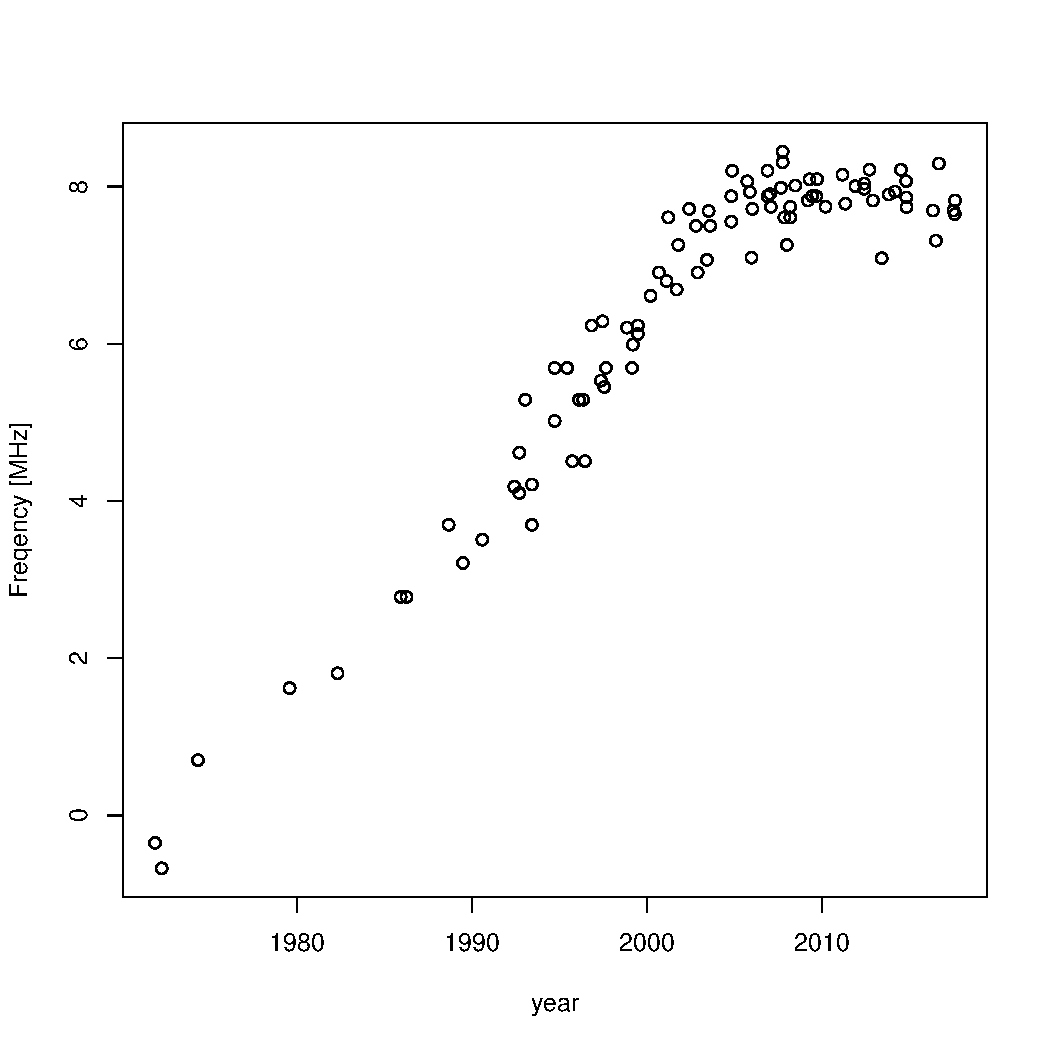
\includegraphics[width=\maxwidth]{figure/unnamed-chunk-1-1} 

\end{knitrout}

\begin{knitrout}
\definecolor{shadecolor}{rgb}{0.969, 0.969, 0.969}\color{fgcolor}\begin{kframe}
\begin{alltt}
\hlkwd{library}\hlstd{(mgcv)}
\end{alltt}


{\ttfamily\noindent\itshape\color{messagecolor}{\#\# Loading required package: nlme}}

{\ttfamily\noindent\itshape\color{messagecolor}{\#\# This is mgcv 1.8-29. For overview type 'help("{}mgcv-package"{})'.}}\begin{alltt}
\hlstd{fit} \hlkwb{<-} \hlkwd{gam}\hlstd{(}\hlkwd{log}\hlstd{(freq)} \hlopt{~} \hlkwd{s}\hlstd{(year),} \hlkwc{data} \hlstd{= data)}
\hlkwd{plot}\hlstd{(}\hlkwd{log}\hlstd{(freq)} \hlopt{~} \hlstd{year,} \hlkwc{data} \hlstd{= data,} \hlkwc{ylab} \hlstd{=} \hlstr{"Freqency [MHz]"}\hlstd{)}
\hlkwd{lines}\hlstd{(data}\hlopt{$}\hlstd{year,}\hlkwd{predict}\hlstd{(fit),} \hlkwc{col} \hlstd{=} \hlstr{"red"}\hlstd{,} \hlkwc{lwd} \hlstd{=} \hlnum{2}\hlstd{)}
\end{alltt}
\end{kframe}
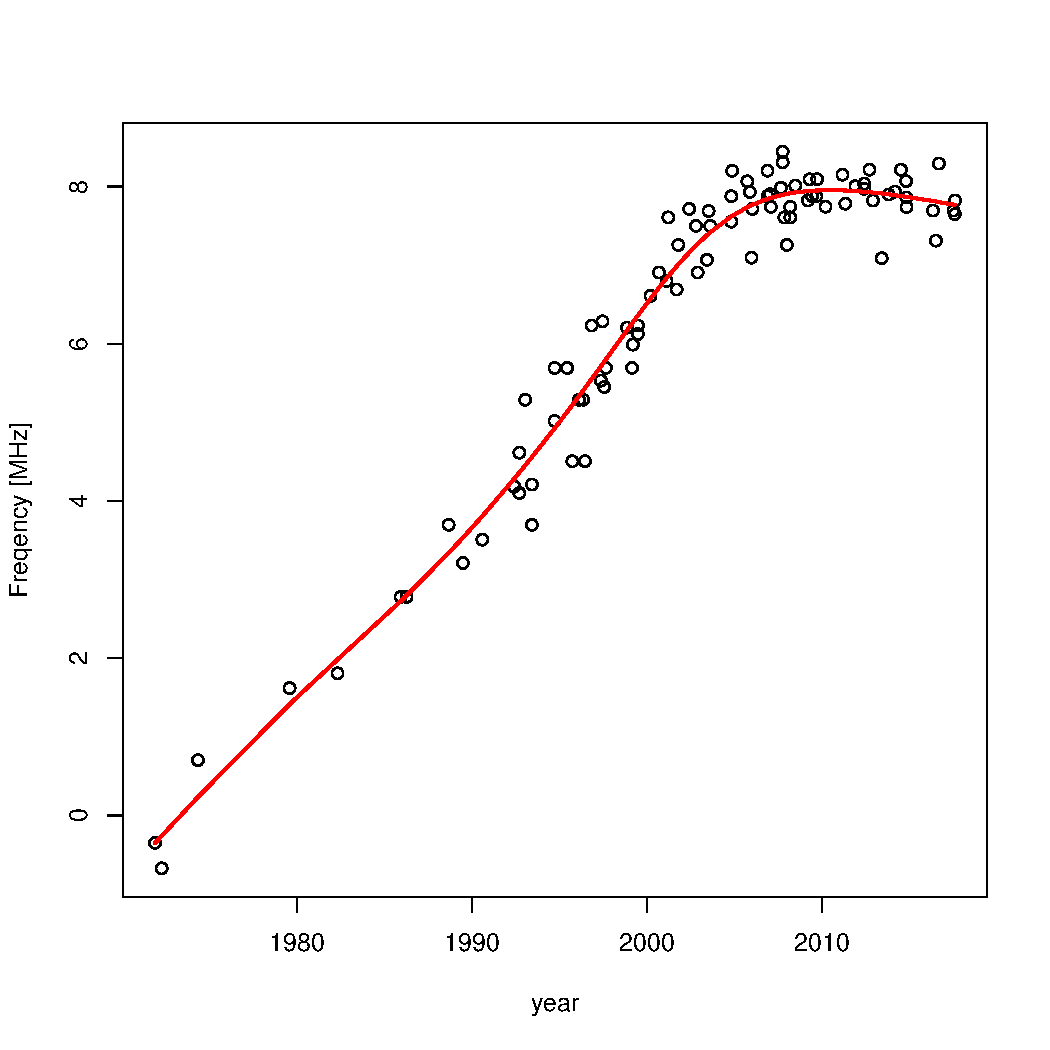
\includegraphics[width=\maxwidth]{figure/unnamed-chunk-2-1} 

\end{knitrout}


\begin{knitrout}
\definecolor{shadecolor}{rgb}{0.969, 0.969, 0.969}\color{fgcolor}\begin{kframe}
\begin{alltt}
\hlkwd{summary}\hlstd{(fit)}
\end{alltt}
\begin{verbatim}
## 
## Family: gaussian 
## Link function: identity 
## 
## Formula:
## log(freq) ~ s(year)
## 
## Parametric coefficients:
##             Estimate Std. Error t value Pr(>|t|)    
## (Intercept)  6.45383    0.03913     165   <2e-16 ***
## ---
## Signif. codes:  0 '***' 0.001 '**' 0.01 '*' 0.05 '.' 0.1 ' ' 1
## 
## Approximate significance of smooth terms:
##           edf Ref.df     F p-value    
## s(year) 5.266  6.378 413.3  <2e-16 ***
## ---
## Signif. codes:  0 '***' 0.001 '**' 0.01 '*' 0.05 '.' 0.1 ' ' 1
## 
## R-sq.(adj) =  0.967   Deviance explained = 96.9%
## GCV = 0.14808  Scale est. = 0.13777   n = 90
\end{verbatim}
\end{kframe}
\end{knitrout}



\end{document}
